\chapter{Metodologia}
\label{cap:ident}



\index{exemplo de figura}
Exemplo de figura na Fig.~\ref{fig:exemploFig}.
\begin{figure}[ht!]
	\center
	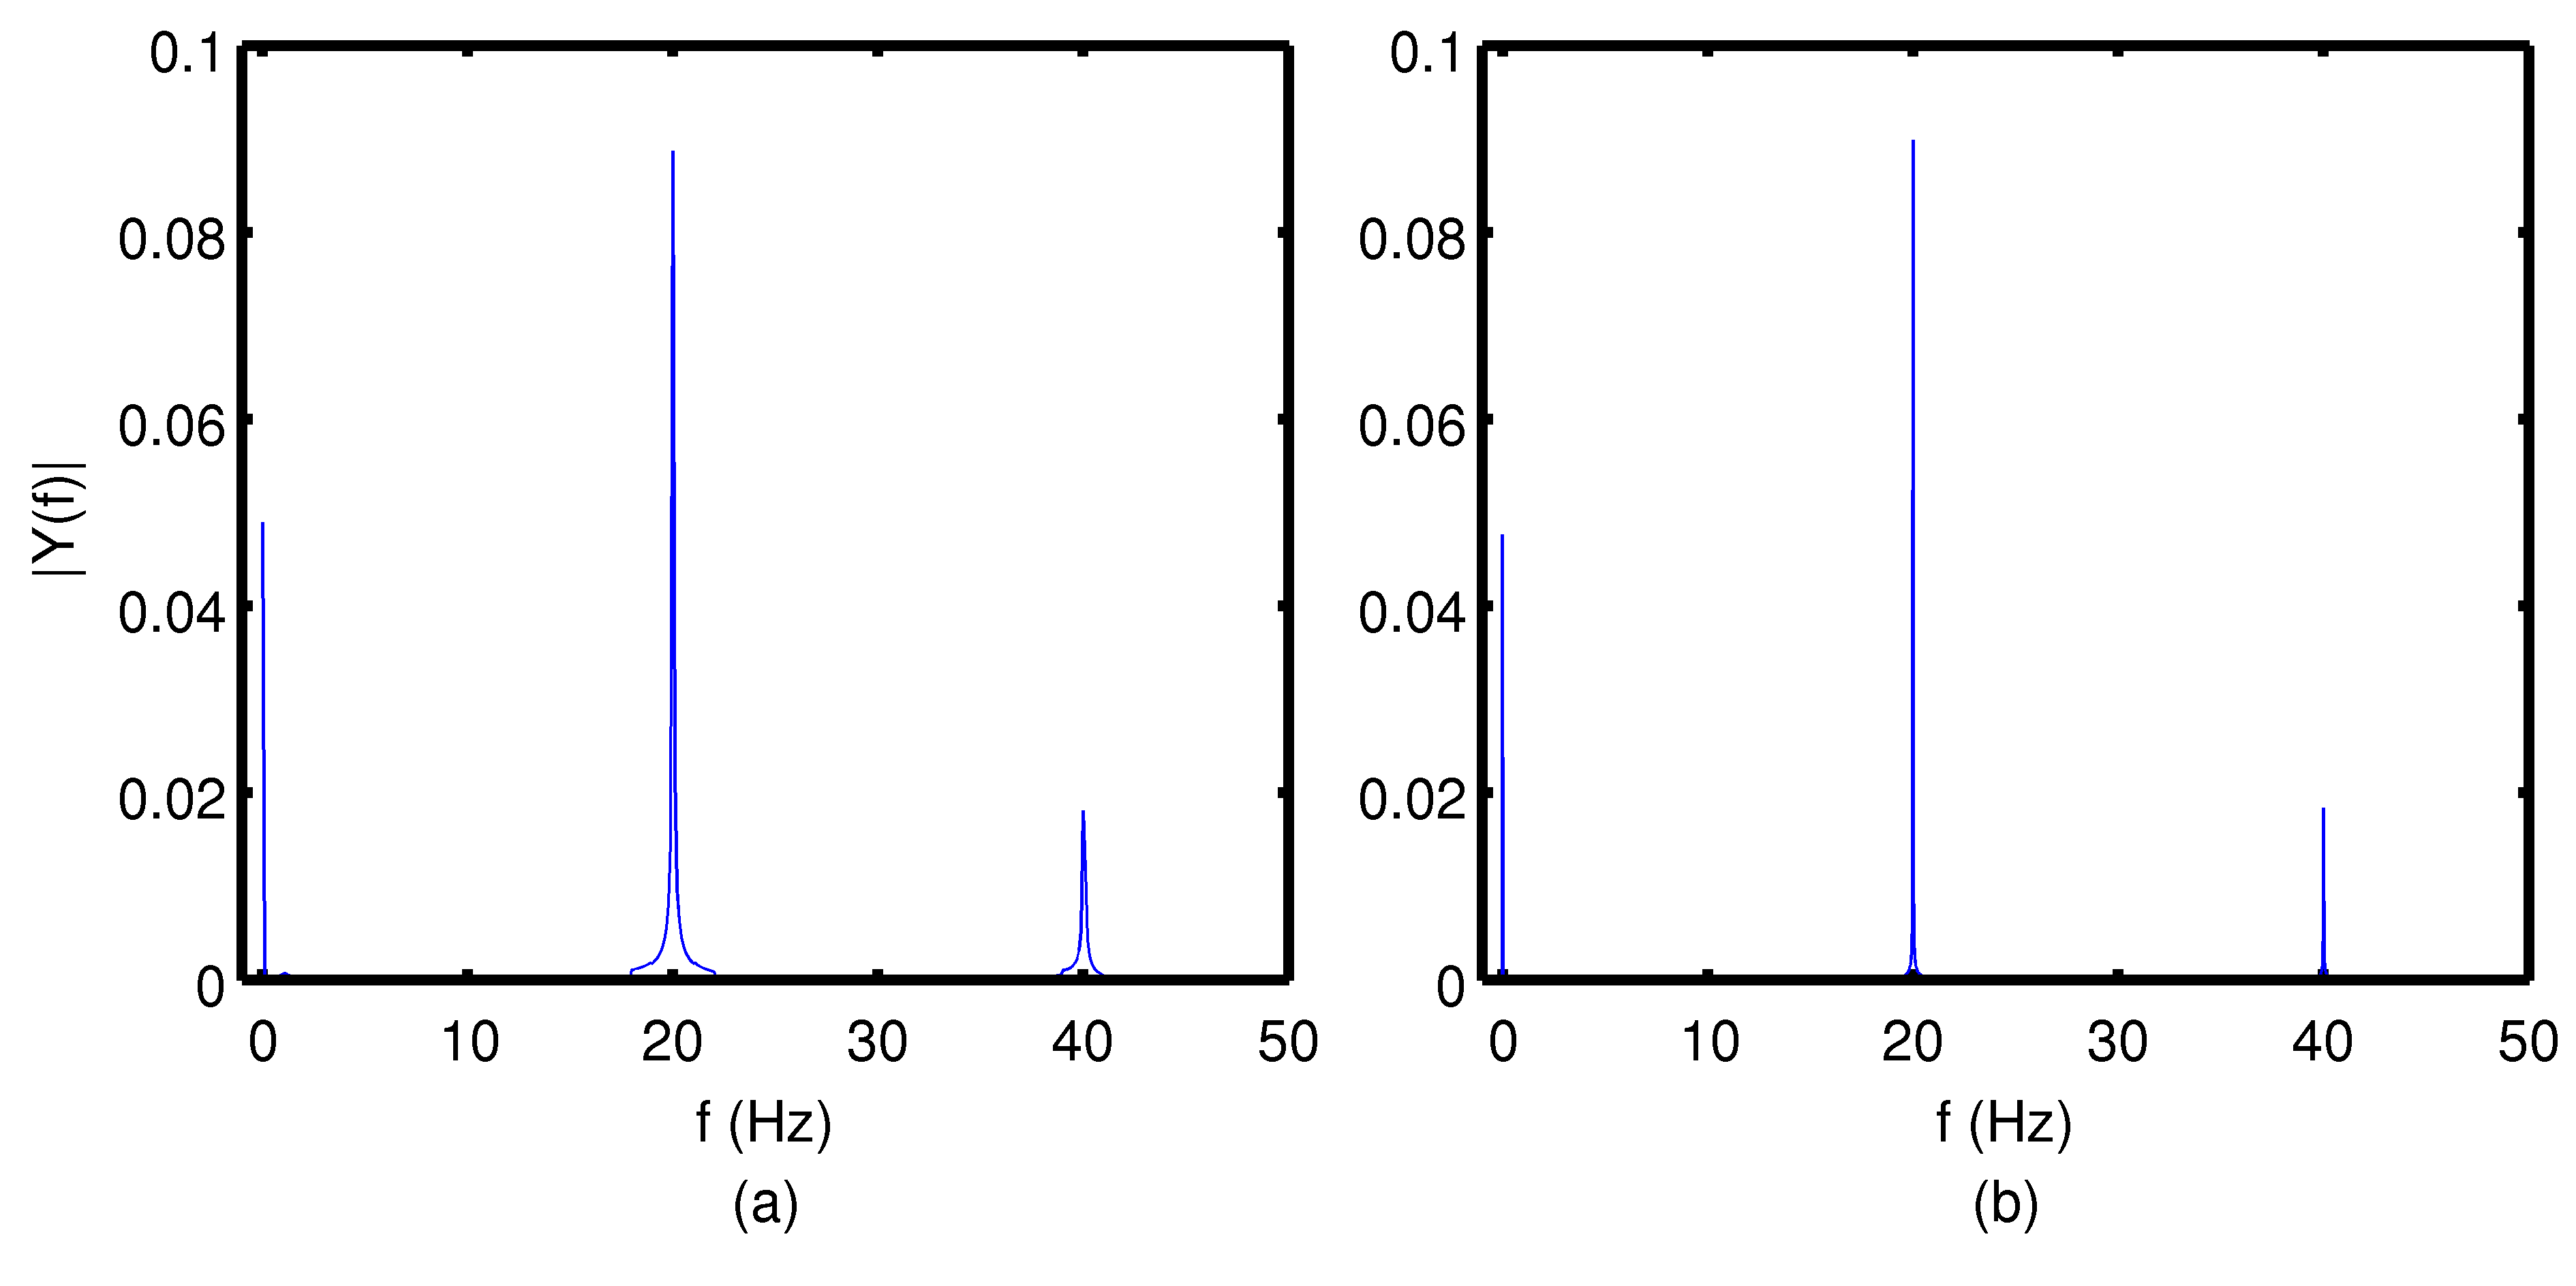
\includegraphics[scale=0.6]{NOFRFExample.png}
	\caption{Exemplo de Figura.}
	\label{fig:exemploFig}
\end{figure}


\index{Exemplo de equa��o}
Exemplo de Equa��o na equa��o~\eqref{eq:exemplo}:
\begin{equation}
  \A = \X + 2
  \label{eq:exemplo}
\end{equation}
 


\section{Mostrando Algoritmo}


\index{Exemplo de algoritmo}
\begin{figure}[!h]
\lstset{language=Matlab, backgroundcolor=\color{gray!10}, keywords=[ 12 ]{func1, indice, naoPertence, para, tamanho, maximo, de, a, se, devolve, soma, e},linewidth=0.95\linewidth,literate={:=}{{$\gets$}}1 {<=}{{$\leqslant$}}1 {>=}{{$\geqslant$}}1 {<>}{{$\neq$}}1 {rho}{{$\rho$}}1   {ws}{{$ws$}}1 {w}{{$w$}}1 {gs_m}{{$gs_m$}}1 {^T}{{$^T$}}1 {^2}{{$^2$}}1 {_s}{{$_s$}}1 {theta}{{$\beta$}}1 {pmatrix}{{\ref{eq:pmatrix}}}1 {^-1}{{$^{-1}$}}1}

\begin{center}
\begin{lstlisting}[frame=single]
func1(param1, param2){
	x := 0
	para (i de 1 a 10){
		x := x + param1 + param2;
	}
	devolve x;	
}
\end{lstlisting}
\end{center}
\vspace{-1.3em}
\caption[Exemplo de Algoritmo]{Exemplo de Algoritmo.}
\label{fig:frols}
\end{figure}

% A matriz $p$, mostrada na Equa��o~\eqref{eq:pmatrix}, quando o modelo segue a representa��o polinomial (Equa��o~\eqref{eq:narmaxpolmodel}), pode ser montada usando o algoritmo na Figura~\ref{fig:pmatrizbuild}. Apesar de parecer simples a montagem desta matriz, achar uma forma geral para o algoritmo n�o foi trivial.  
%

Um exemplo de Tabela � mostrado na Tabela~\ref{tab:exemploTabela}.

\index{Exemplo de Tabela}
\begin{table}[ht!]
\caption{Exemplo de Tabela}
\label{tab:exemploTabela}
\centering
   \begin{tabular}{lrrr}\hline 
	A&B&C&D \\ \hline 
	y(k-1)&2.59e+00&2.44e+00&2.28e+00  \\ 
	y(k-2)&-2.35e+00&-2.12e+00&-1.79e+00  \\ 	
	\hline
    \end{tabular}
\end{table}   





